
\newpage
\subsection{Numerical Experiments}

Same kind of mesh of the section \ref{r2_verification} can be used. The boundary conditions are similar to the rank 1 case, but the Gaussian distribution is now applied as a Neumann boundary condition, this is:

\begin{equation*}
D \nabla \phi \cdot \hat{n} = \dfrac{ e^{\frac{-(x - \mu)^2}{2 \sigma^2}}}{2 \pi \sqrt{2 \pi}} + \dfrac{ e^{\frac{-(y - \mu)^2}{2 \sigma^2}}}{2 \pi \sqrt{2 \pi}} \text{ on left and bottom boundary}
\end{equation*}

In first place, the homogeneous case can be calculated, just for verification effects. In the figure \ref{fig:error_homo} the evolution in time of the error can be appreciated and note that the values stay below the machine precision level, as is expected.

The domain for the examples of this section is a $6 \times 6 [mm^2]$ square. The mesh used for the homogenized problem can be seen in the figure \ref{fig:mesh_h_r2}, that have 84 DOF's.

\begin{figure}[H]
\centering
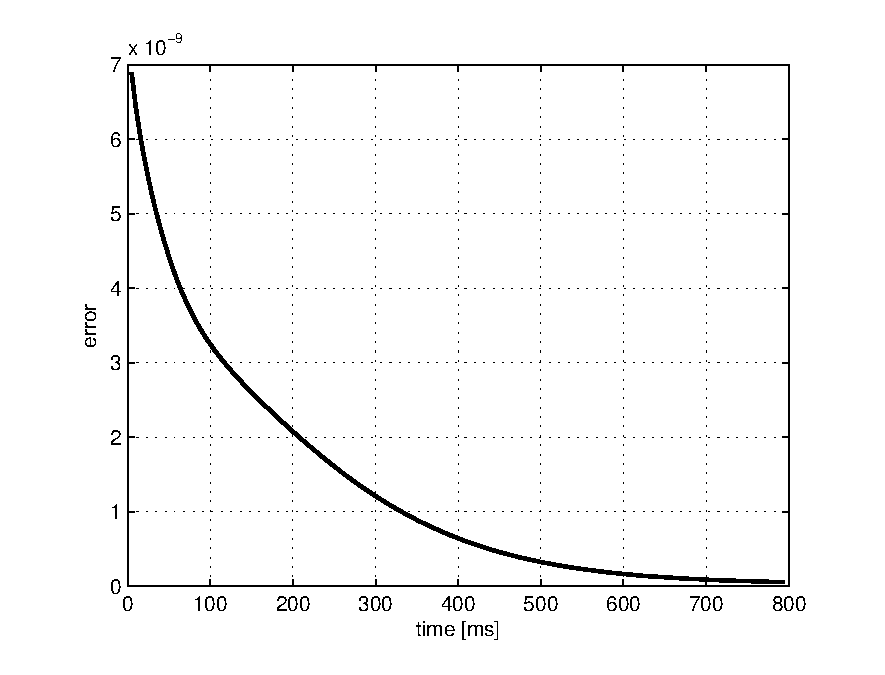
\includegraphics[height = 6 cm]{fig/theorem_verification_r2_error_homo}
\caption{temporal evolution of the error, considering an homogeneous media (machine precision level error)}\label{fig:error_homo}
\end{figure}

\begin{figure}[H]
\centering
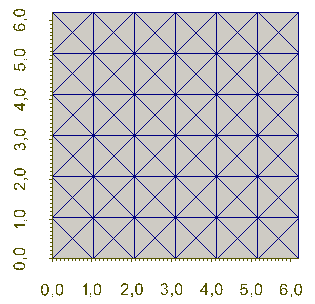
\includegraphics[height = 6.2 cm]{fig/theorem_verification_r2_exp_mesh_h}
\caption{mesh for homogenized problem in experiments \# 1 and \# 2.} \label{fig:mesh_h_r2}
\end{figure}


Now, in the table \ref{fig:exp_r2_setup} the set-up for the two proceeding experiments is shown.

\begin{table}[H]
\centering
\label{tab:geometric_setup_diff_r2}
\begin{tabular}{@{}cccccccc@{}}
\toprule
       & \# DOF's & a {[}mm{]} & b {[}mm{]} & $\theta_c$ & $\theta_f$ & $\beta$   & $\gamma$ \\ \midrule
Exp. 1 & 268028   & 0.1        & 1          & 0.2        & 0.5        & 0.01      & 5        \\
Exp. 2 & 232324   & 0.1        & 1          & 0.4        & 0.5        & $10^{-5}$ & 5        \\ \bottomrule
\end{tabular}
\caption{configuration for numerical experiments.} \label{fig:exp_r2_setup}
\end{table}

With all this, we are in order to perform the FEM discretization and resolution of the equation \ref{eq:diff_dynamic_weak_form}. To solve the linear system was used Gaussian elimination, and the assemble of the matrix was realized at each time step. In the figure \ref{fig:verification-r2ex1} and \ref{fig:error_diff_r2} the solution and error of the first configuration are shown, as the same is presented in figures \ref{fig:verification-r2ex2} and \ref{fig:error_diff_r2_ex2} for the second configuration.

\subsubsection*{Results of Experiment \# 1: Moderated ``Fibrosis''}

\begin{figure}[H]
\centering
\subfigure{
    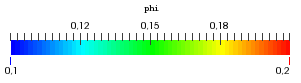
\includegraphics[height = 1.2 cm]{fig/theorem_verification_r2_exp2_colorbar}} \\
\subfigure[5 ms]{
    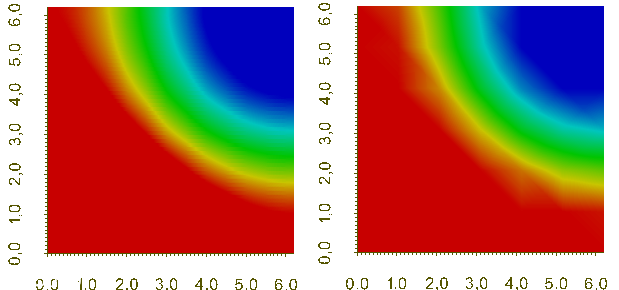
\includegraphics[height = 5.2 cm]{fig/theorem_verification_r2_exp1_5ms}} 
\subfigure[55 ms]{
    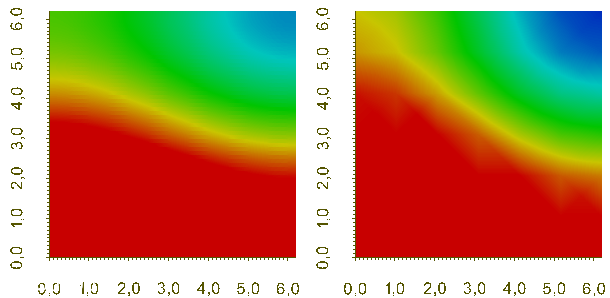
\includegraphics[height = 5.5 cm]{fig/theorem_verification_r2_exp1_55ms}}    
\subfigure[100 ms]{
    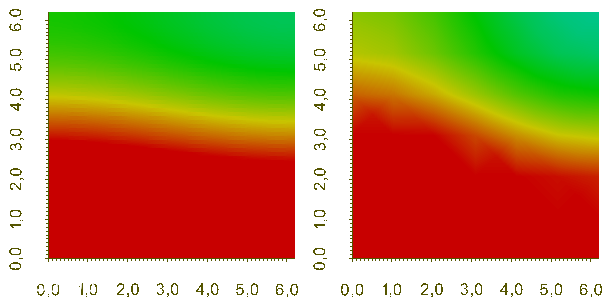
\includegraphics[height = 5.5 cm]{fig/theorem_verification_r2_exp1_100ms}}     
\end{figure}

\begin{figure}[H]
\centering
\subfigure[430 ms]{
    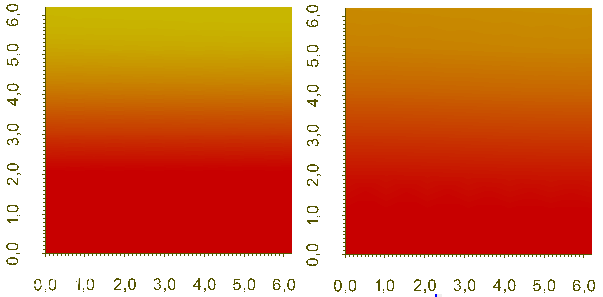
\includegraphics[height = 5.5 cm]{fig/theorem_verification_r2_exp1_430ms}} 
\subfigure[800 ms]{
    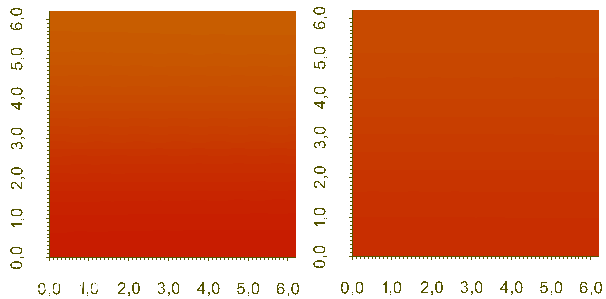
\includegraphics[height = 5.5 cm]{fig/theorem_verification_r2_exp1_800ms}}
\caption{temporal evolution of the solution for the exact problem (left) and homogenized problem (rigth)}\label{fig:verification-r2ex1}
\end{figure}

\begin{figure}[H]
\centering
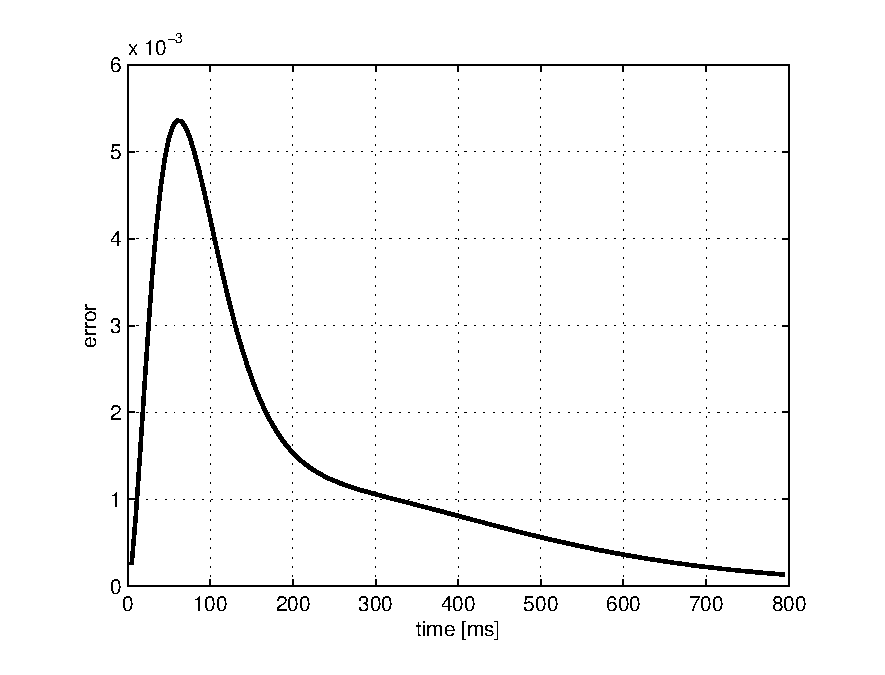
\includegraphics[height = 6 cm]{fig/theorem_verification_r2_exp1_error}
\caption{error v/s time for experiment \# 1} \label{fig:error_diff_r2}
\end{figure}

\newpage 
\subsubsection*{Results of Experiment \# 2: High ``Fibrosis''}

\begin{figure}[H]
\centering
\subfigure{
    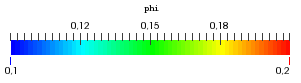
\includegraphics[height = 1.2 cm]{fig/theorem_verification_r2_exp2_colorbar}} \\
\subfigure[5 ms]{
    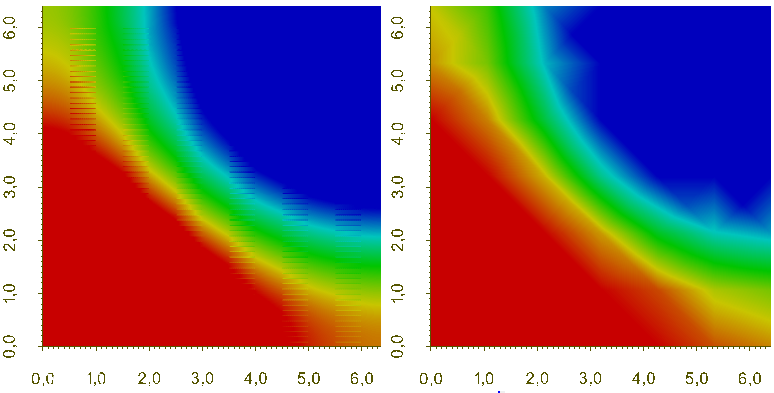
\includegraphics[height = 5.5 cm]{fig/theorem_verification_r2_exp2_5ms}} 
\subfigure[70 ms]{
    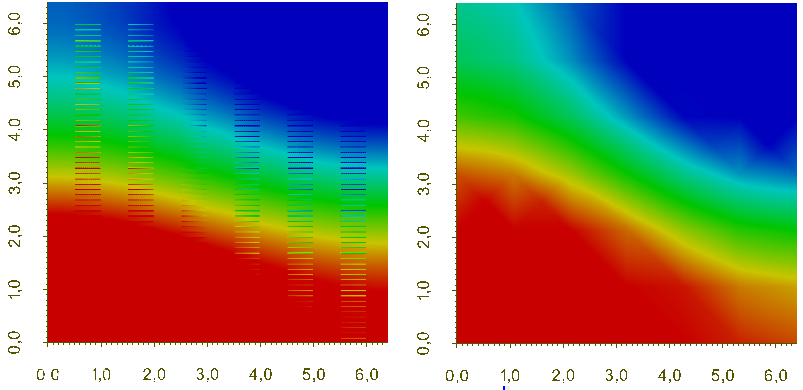
\includegraphics[height = 5.5 cm]{fig/theorem_verification_r2_exp2_70ms}}    
\subfigure[258 ms]{
    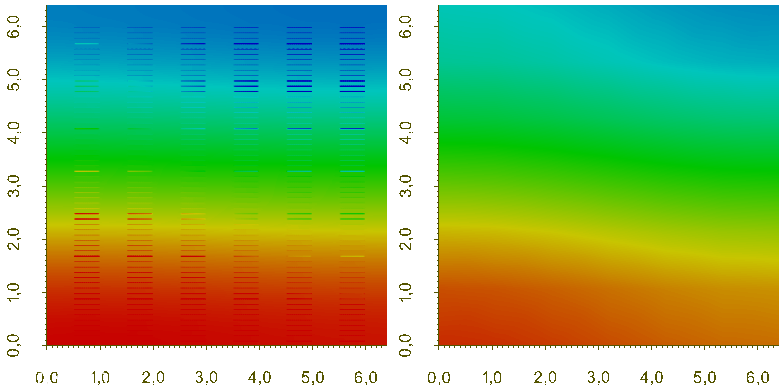
\includegraphics[height = 5.5 cm]{fig/theorem_verification_r2_exp2_258ms}}     
\end{figure}

\begin{figure}[H]
\centering
\subfigure[400 ms]{
    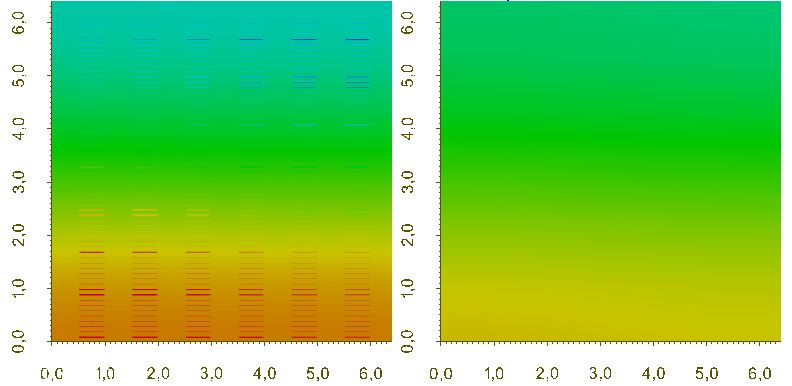
\includegraphics[height = 5.5 cm]{fig/theorem_verification_r2_exp2_400ms}} 
\subfigure[800 ms]{
    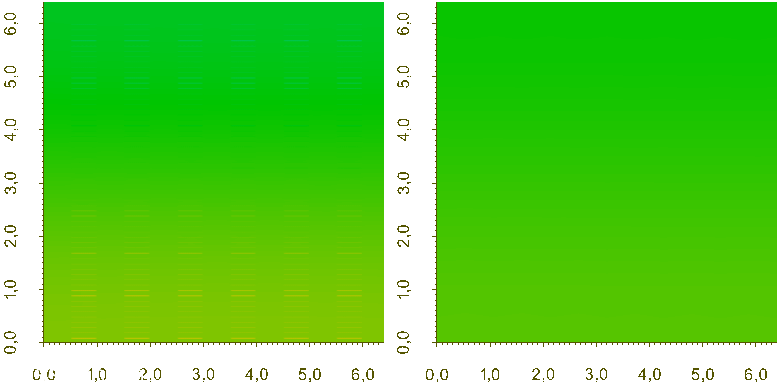
\includegraphics[height = 5.5 cm]{fig/theorem_verification_r2_exp2_800ms}}
\caption{temporal evolution of the solution for the exact problem (left) and homogenized problem (rigth)}\label{fig:verification-r2ex2}
\end{figure}

\begin{figure}[H]
\centering
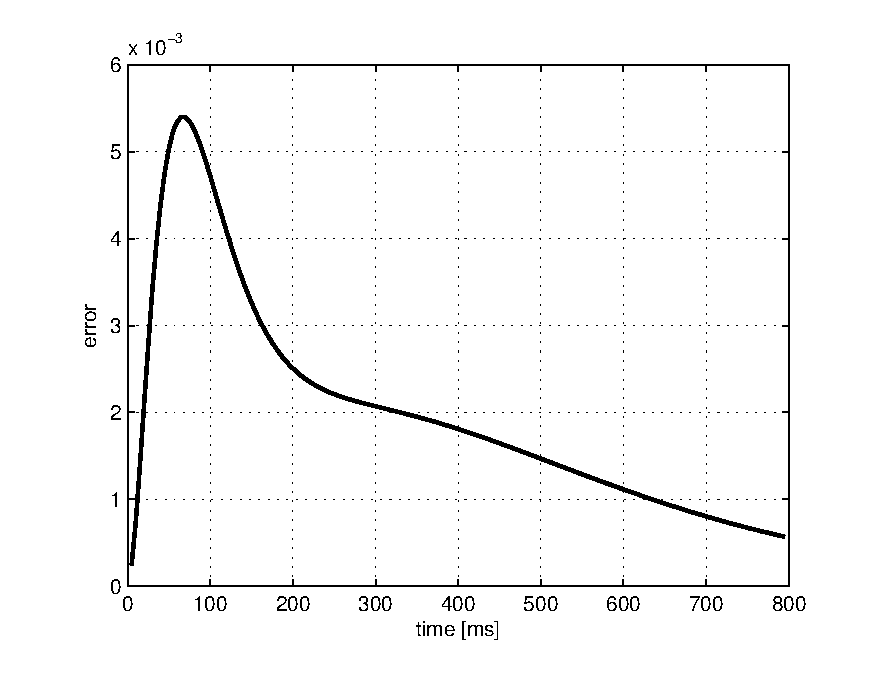
\includegraphics[height = 6 cm]{fig/theorem_verification_r2_exp2_error}
\caption{error v/s time for experiment \# 2}\label{fig:error_diff_r2_ex2}
\end{figure}

\newpage
\section{Beyond the Theorem: A first approach to model diffuse fibrosis}

\white{....} Now, can be done a first approach to simulate diffuse fibrosis. In order to do this, the FitzHugh-Nagumo model can be introduced in the monodomain equations (\ref{eq:MDE}), obtaining:  

\begin{equation}
\arraycolsep=1.4pt\def\arraystretch{2.2}
\left\lbrace
\begin{array}{lr}
\dfrac{\partial \phi}{ \partial t} - div(D \nabla \phi) = c_1 \phi (\phi - \alpha)(1 - \phi) - c_2 r \\ 
\dfrac{\partial r}{\partial t} = c_2 (\phi - rd)\\
\phi = \overline{\phi} & \text{ on } \Gamma_D ~~ \forall t \geqslant 0 \\
D \nabla \phi \cdot  \hat{n}= g & \text{ on } \Gamma_N ~~ \forall t \geqslant 0 \\
\phi = \phi_0 &\text{ for } t = 0 ~~ \text{ on } \Omega  \\
r = r_0 &\text{ for } t = 0 ~~ \text{ on } \Omega \\
\end{array}
\right.
\end{equation}

For the homogenized problem it used same diffusion tensor as the previous problems. Notice that for this problem the necessary conditions for the homogenization theorem (\ref{eq:homogenization_rank1}) are violated, but still the same tensor will be used. This last is known as a \textsl{surrogate} model. \\

As in the section \ref{sec:dinamyc_case}, we can solve the PDEs by the finite element method, but first discretize the time derivative by a finite difference approximation.

\subsection{Derivation of Time-Discretization Squeme}


\white{....} Let's multiply both sides of FitzHugh-Nagumo equations by $\phi$ and $r$, where corresponds.

\begin{equation*}
\phi \dfrac{\partial \phi}{ \partial t}  = \{ c_1 \phi (\phi - \alpha)(1 - \phi) - c_2 r \}\phi
\end{equation*}

\begin{equation*}
r \dfrac{\partial r}{\partial t}  = \{ c_2 (\phi - rd) \} r
\end{equation*}

Now, adding both equations and considering that:
\begin{equation*}
\phi \dfrac{\partial \phi}{ \partial t} + r \dfrac{\partial r}{\partial t} = \frac{1}{2} \frac{d}{dt} \left(\phi^2 + r^2 \right):= E
\end{equation*}

\noindent its obtained:

\begin{equation}
E = c_1 (1 + \alpha) \phi^3 - c_1 (\alpha \phi^2 +  \phi^4) -c_2 d r^2 \label{eq:total_energy}
\end{equation}

\noindent where the coupling term $c_2 \phi r$ has been cancelled. The E magnitude can be interpreted as the total energy of the system. In this context, results natural the anulation of the coupling term, since the energy cannot be generated in the ``interface'' of the system. Note that nearly all terms in the right side of equation (\ref{eq:total_energy}) dissipates energy from the system, in exception of $c_1 (1 + \alpha) \phi^3$, that constitutes a potential instability source. So, the balance between this last and the others terms conditions the decay of the solution.

Its desirable that the discretized version of the continuous system preserves the stability properties of it. To evaluate this, a general $\theta-$squeme can be used for the time discretization of the EDO, while a ``$\beta-$squeme'' can be used for the PDE, where the discretization has been done in order to obtain a linear problem:

\begin{equation}
\arraycolsep=1.4pt\def\arraystretch{2.2}
\begin{array}{llr}
\dfrac{r^{n+1}-r^n}{\Delta t} 
= &\{ \beta (c_2 \phi^{n + 1}) + (1 - \beta  )(c_2 \phi^{n + 1}) \} 
- \{ \theta  (c_2 d r^{n + 1}) + (1 - \theta )c_2 d r^{n} \} \\

\dfrac{\phi^{n+1} - \phi^n}{\Delta t}
= &c_1(1 + \alpha)\phi^n \{ \beta (\phi^{n+1})^2 + (1 - \beta) (\phi^{n})^2 \} 
- c_1 \alpha \{ \beta \phi^{n+1}  + (1 - \beta) \phi^n \} 
- c_1 (\phi^n)^2 \{ \beta \phi^{n+1} \} \\
 &- c_2 \{\theta r^{n+1} + (1 - \theta) r^{n} \}
\end{array} \label{eq:teta_esquema_MDE}
\end{equation}

\noindent where $\phi^{n}$ and $r^{n}$ are the potential and the internal variable at the time step n, respectively. There exist, for instance, the following cases:

\begin{itemize}
\item $\theta = \beta = 0 \rightarrow$  explicit (forward Euler) and uncoupled problem.
\item $\theta = 1$ and $\beta = 1 \rightarrow$ implicit (backward Euler) and coupled problem.
\item $\theta = 1/2$ and $\beta = 1/2 \rightarrow$ implicit (Crank-Nicolson) and coupled problem.  
\end{itemize}

In general, for $\beta$ and $\theta$ greaters than a half, a implicit squeme will be obtained. To understand the ``energy'' change of the discrete system in time the equations (\ref{eq:teta_esquema_MDE}) are multiplied by $r^{n + \theta}$ and $\phi^{n + \beta}$ up and down, respectively, were the notation $a^{n + \theta} := \theta a^{n+1} + (1 - \theta), a^n$ has been adopted. Now, after some algebra arrangements its obtained:

\begin{equation}
\arraycolsep=1.4pt\def\arraystretch{2.2}
\begin{array}{llr}
\overline{E}:= & \dfrac{1}{2} \dfrac{r^{n+1}}{dt} - \dfrac{1}{2} \dfrac{r^{n}}{dt} + \dfrac{1}{2} \dfrac{\phi^{n+1}}{\Delta t} - \dfrac{1}{2} \dfrac{\phi^{n}}{\Delta t} \\

& = c_2 \phi^{n + \beta} r^{n + \theta} 
- c_2 d (r^{n + \theta})^2 
- \red{(\theta - \frac{1}{2}) \frac{1}{\Delta t} (r^{n+1} - r^n)^2} 
+ c_1 (1 + \alpha) \phi^n (\phi^{n + \beta})^2 \\
& - c_1 \alpha (\phi^{n + \beta})^{2}
- c_1 (\phi^n)^2 (\phi^{n + \beta})^2
- c_2 r^{n + \theta} v^{n + \beta}
- \red{(\beta - \frac{1}{2}) \frac{1}{\Delta t} (\phi^{n+1} - \phi^n)^2 }
\end{array}
\end{equation}

\noindent where $\overline{E}$ is the total ``\textsl{numerical energy}'' of the system. Note that the terms in red are not present in the continuos stability analisys, so is desirable, in order to preserve stability properties of the continuous system, that this term doesn't add energy to the system, which is achieved simply considering $\theta \geqslant 0.5$ and $\beta \geqslant 0.5$.

Finally, the following \textsl{semi-implicit} squeme is adopted (\red{como se asegura que este esquema no inyecta energía numérica al sistema? (no respeta regla deducida en parrafo anterior)}):

\begin{equation}
\arraycolsep=1.4pt\def\arraystretch{2.2}
\begin{array}{llr}
\dfrac{r^{n+1} - r^n}{\Delta t} = c_2 \phi^n - c_2 d r^{n+1} \\
\dfrac{\phi^{n+1} - \phi^n}{\Delta t} = c_1 (1 + \alpha) (\phi^n)^2 - c_1 \alpha \phi^{n+1} - c_1 (\phi^n)^3 + div(D \nabla \phi^{n+1})
\end{array}
\end{equation}

\noindent where all the non-linear terms has been left explicit, and the linear ones has been left implicit. Also, the potential in the internal FHN equation has been left explicit, in order to finally obtain a linear and uncoupled problem. Note that the diffusion term has been added and was left implicit(\red{porqué?}).

\subsection{Weak Form of MDE+FHN}

\white{....} Now, the weak variational form of the time-discretized PDE must to be written in order to perform a FEM discretization of the space for each time step $n$. So, the variational form of the time step $n$ as $a_{n + 1} (\phi^{n + 1}, v) = L(v)$ and the FHN internal equation are written as follows:

\begin{equation*}
r^{n+1} = r^n + \Delta t c_2 (\phi^n - r^{n+1} d)
\end{equation*}
\begin{equation}
a_{n+1} (\phi^{n + 1}, v) = \int_{\Omega} (1 + \Delta t c_1 \alpha) \phi^{n+1} v d \Omega + \Delta t \int_{\Omega} D \nabla \phi^{n+1} \nabla v d \Omega \label{eq:esquema_definitivo}
\end{equation}
\begin{equation*}
L_{n+1}(v) = \int_{\Omega} \phi^n v d \Omega + \Delta t \int_\Omega \{ c_1(1 + \alpha)(\phi^n)^2 - c_1 (\phi^n)^3 - c_2 r^{n+1} \} v d \Omega + \Delta t \int_{\Gamma_N} g  v ds 
\end{equation*}



\noindent where the same test functions of the previous examples was used. On the other hand, a explicit squeme can be used, where all the terms are time-discretized with a foward euler squeme. This leads to:

\begin{equation*}
r^{n+1} = r^n + \Delta t c_2 (\phi^n - r^n d)
\end{equation*}

\begin{equation}
a_{n+1}(\phi^{n+1}, v) = \int_{\Omega} \phi^{n+1} v d \Omega + \Delta t \int_{\Omega} D \nabla \phi^{n+1} \nabla v d \Omega \label{eq:esquema_explicito}
\end{equation}

\begin{equation*}
L(v) =  \int_{\Omega} \phi^n v d \Omega + c_1 \phi^n (\phi^n - \alpha)(1 - \phi^n) - c_2 r^{n+1}+ \Delta t \int_{\Gamma_N} g  v ds 
\end{equation*}



\subsection{Numerical Examples}
\subsubsection{Experiment \# 1: A Single Cell}

\white{....} First, a case with a small domain can be verified, where the spatial dependence can be neglected (single cell). In figure \ref{fig:fhn_nofisiologico2} a solutions where an  a implicit (backward) euler scheme is used. As initial conditions are considered $\phi(0) = 0.2 [mV]$ and $r(0) = 0$. The time step can be taken as $\Delta t = 18 [ms]$. To solve the $2 \times 2$ equation system $\vec{F}(\phi_k, r_k) = 0$ for each step a quasi-Newton method is employeed.

\begin{figure}[H]
\centering 
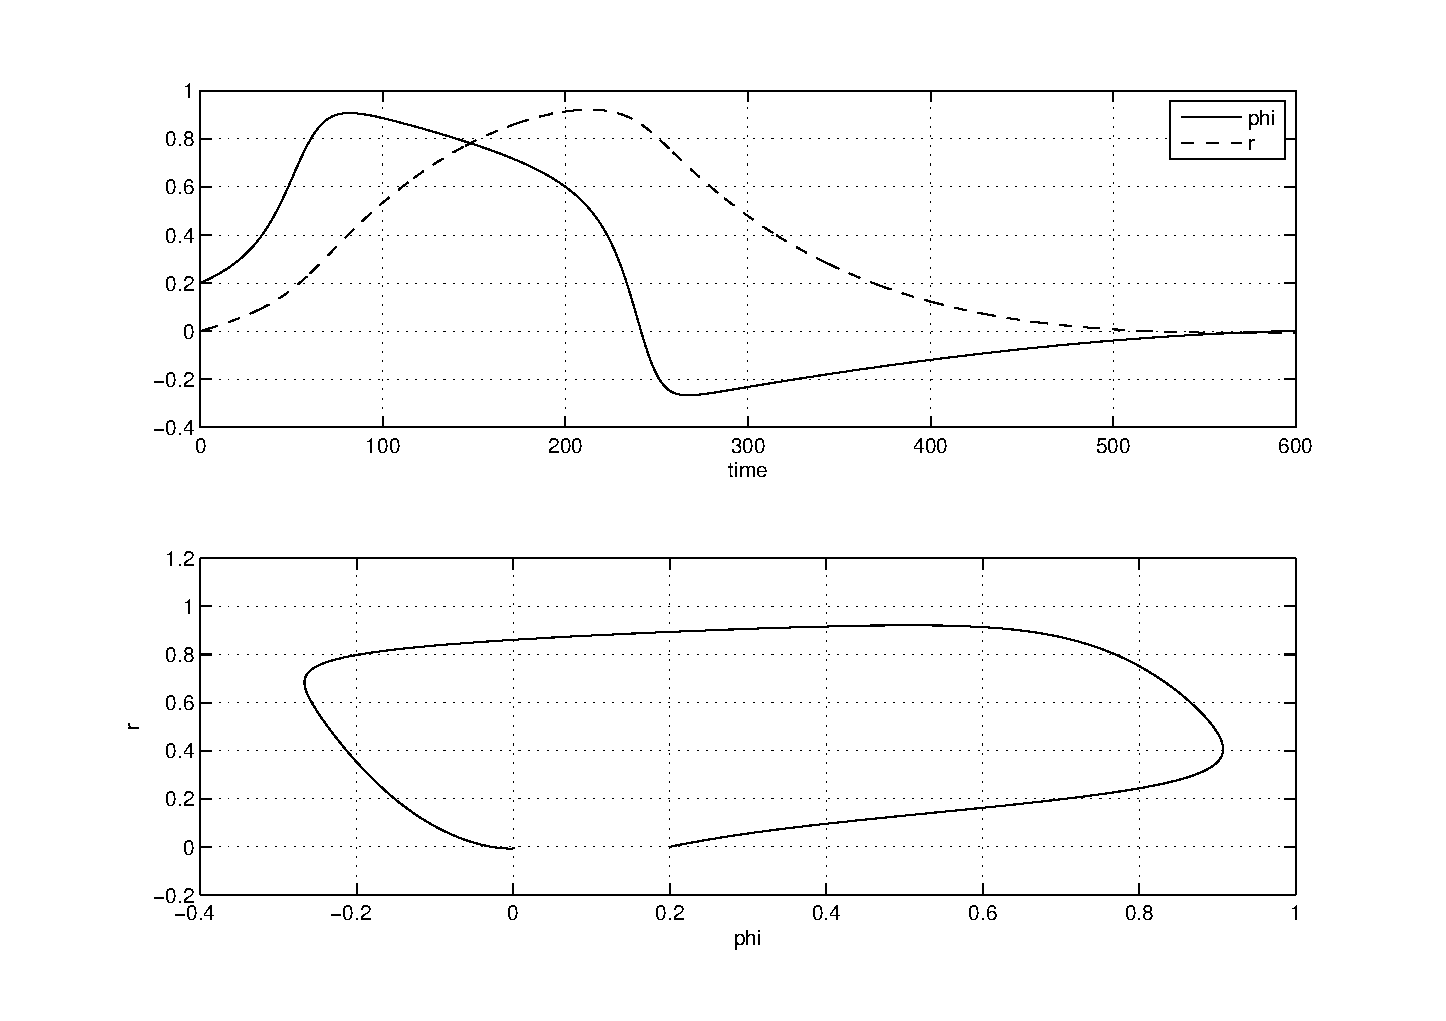
\includegraphics[height = 8.5 cm]{fig/reaction_term-FHN_implicit}
\caption{Numerical solution of the FitzHugh-Namuno equations using $c_1 = 0.175$, $c_2 = 0.03$, $\Delta t = 18 [ms]$, $d = 0.55$ and $\alpha = 0.08$.}
\label{fig:fhn_nofisiologico2}
\end{figure}

\newpage 
\subsubsection{Experiment \# 2: High Fibrosis on Tiny Domain}

\white{....} From here, just the \textsl{semi-implicit} time-discretization (\ref{eq:esquema_definitivo}) will be used, because (\ref{eq:esquema_explicito}) needs too shorts time-steps. Indeed, for this experiment is used $\Delta t = 10 [ms]$, while the explicit problem (\ref{eq:esquema_explicito}) admits a maxium time-step of $0.05 [ms]$ for the same configuration (see table \ref{tab:mde_setup_2}).

\begin{table}[H]
\centering
\begin{tabular}{@{}cccccccc@{}}
\toprule
 \# DOF's & a {[}mm{]} & b {[}mm{]} & $\theta_c$ & $\theta_f$ & $\beta$   & $\gamma$ & $\Delta t$ [ms]\\ \midrule
 328854   & 0.1        & 1          & 0.4        & 0.5        & $10^{-5}$     & 5   & 10     \\ \bottomrule
\end{tabular}
\caption{setup for experiment.} \label{tab:mde_setup_2}
\end{table}

The normalized threshold potential, the excitation rate constant and the other variables of the FHN model has been taken with the same values of the experiment in a single cell. Also the boundary conditions are still the same, but are divided by 10, in order to calibrate it with the reaction parameters. \\

The result of the numerical solution can be apreciated in the figure \ref{fig:mde_ex2}, while the error and computing time is plotted in figures \ref{fig:mde_ex2_error} and \ref{fig:mde_ex2_benchmark}, respectively. Probably, the main reason of the time difference relay on the mesh coarsening for the homogenized problem, which have have 841 DOF's. 

\begin{figure}[H]
\centering
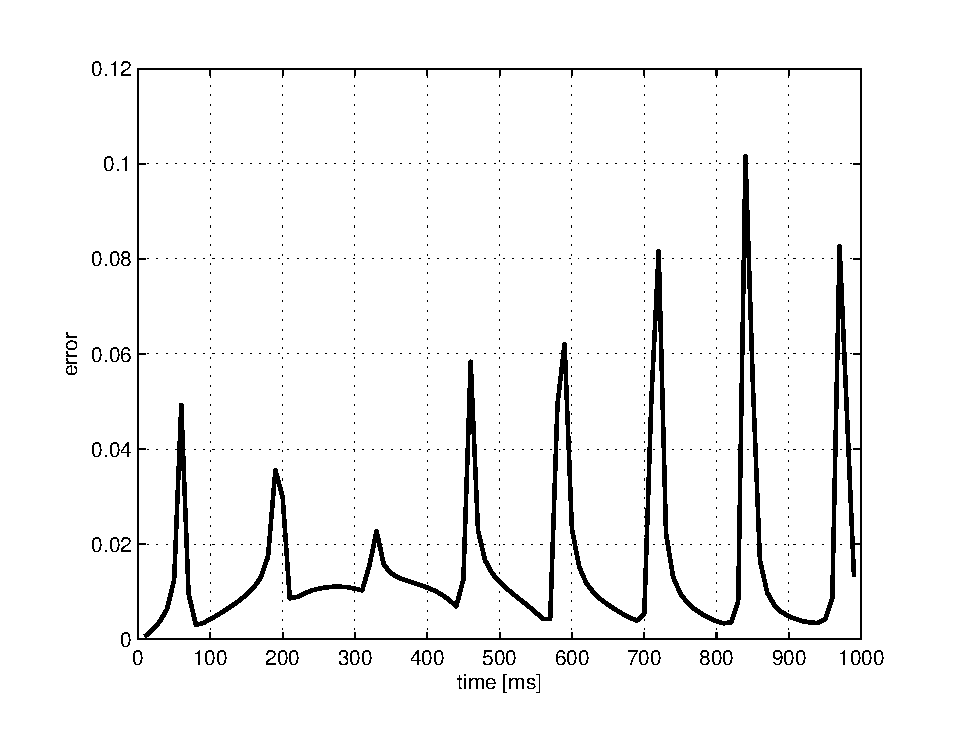
\includegraphics[height = 7 cm]{fig/numerical_example_MDE_exp1_error}
\caption{evolution of the error in time.} \label{fig:mde_ex2_error}
\end{figure}

The assemble of the matrix that doesn't depend of time are assembled just once previous to the time loop. In this assemble process, the exact problem takes 47.18 [seg], while the homogenized takes 0.0171 seg. So, in total, the exact problems takes 193,002 [seg], while the homogenized takes only 1,265 [seg].

\begin{figure}[H]
\centering
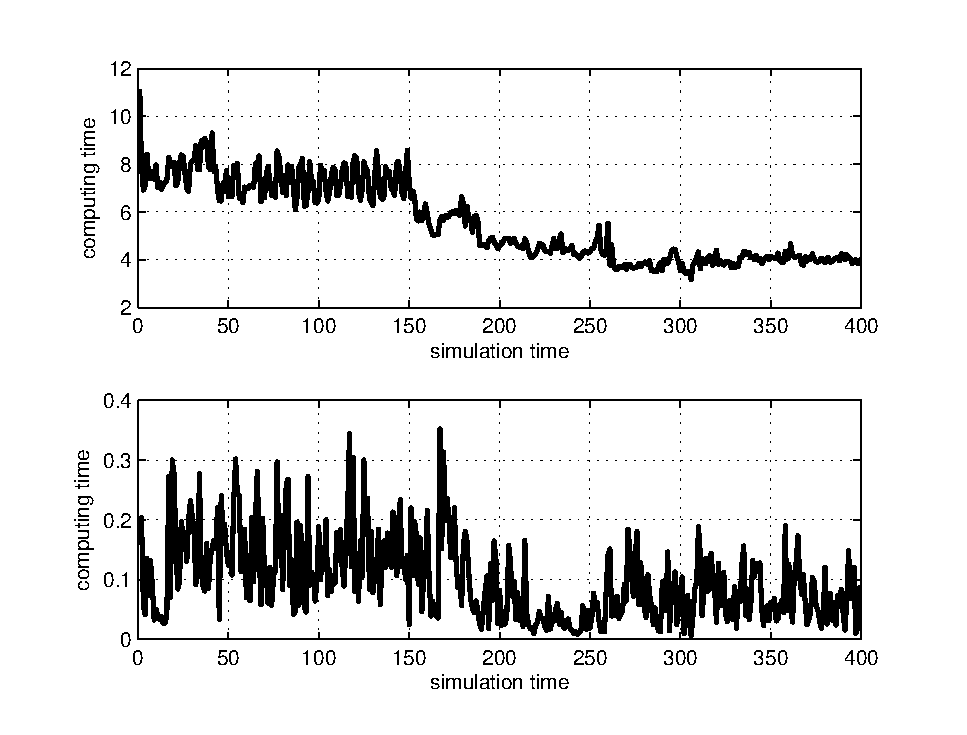
\includegraphics[height = 7 cm]{fig/numerical_example_MDE_exp1_benchmark}
\caption{evolution of computing time.} \label{fig:mde_ex2_benchmark}
\end{figure}

\begin{figure}[H]
\centering
\subfigure{
    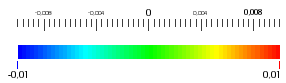
\includegraphics[height = 1.2 cm]{fig/numerical_example_MDE_exp1_colourbar}} \\
\subfigure[30 ms]{
    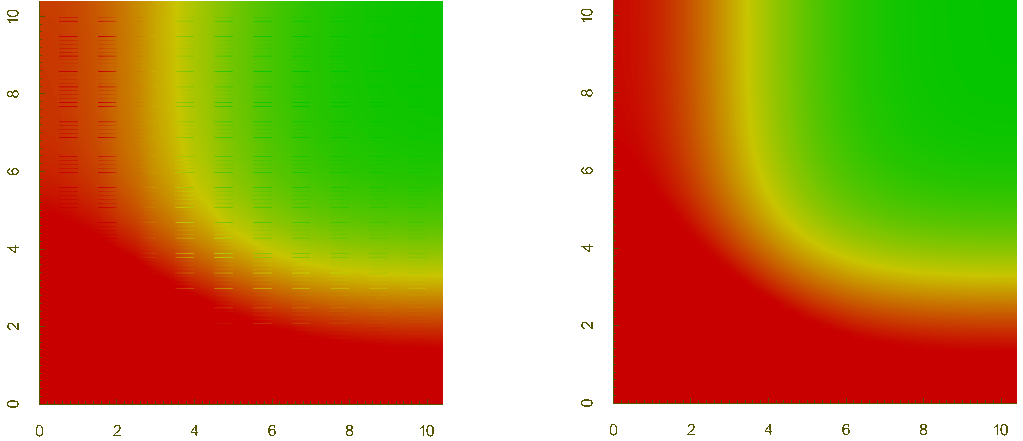
\includegraphics[height = 5 cm]{fig/numerical_example_MDE_exp1_30ms}}
\subfigure[120 ms]{
    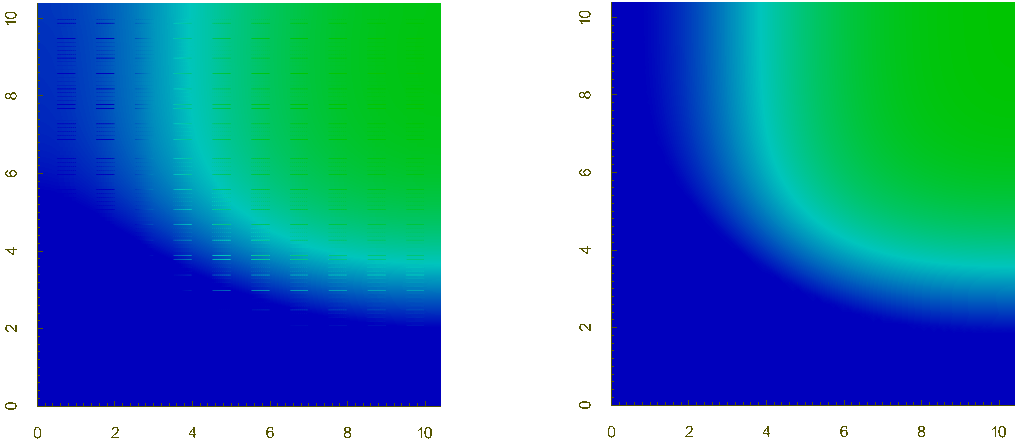
\includegraphics[height = 5 cm]{fig/numerical_example_MDE_exp1_120ms}}      
\end{figure}

\begin{figure}[H]
\centering 
\subfigure[200 ms]{
    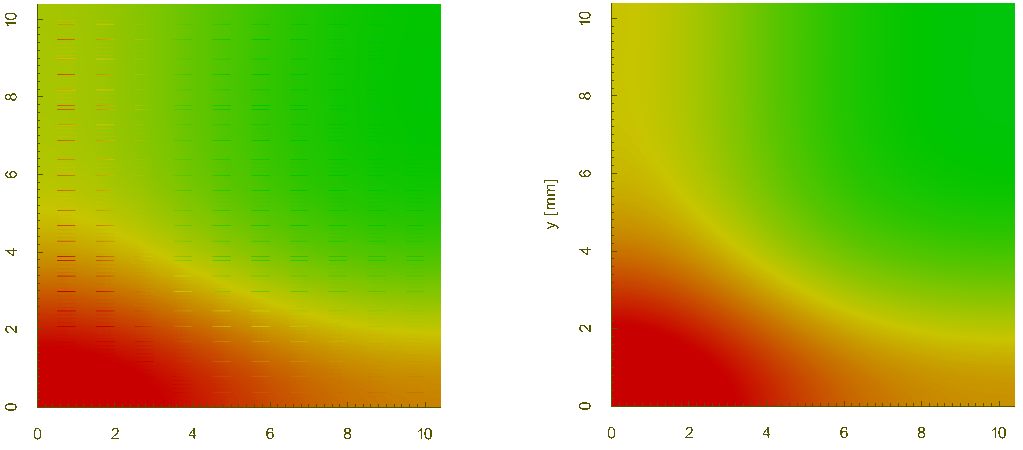
\includegraphics[height = 5.5 cm]{fig/numerical_example_MDE_exp1_200ms}} 
\subfigure[400 ms]{
    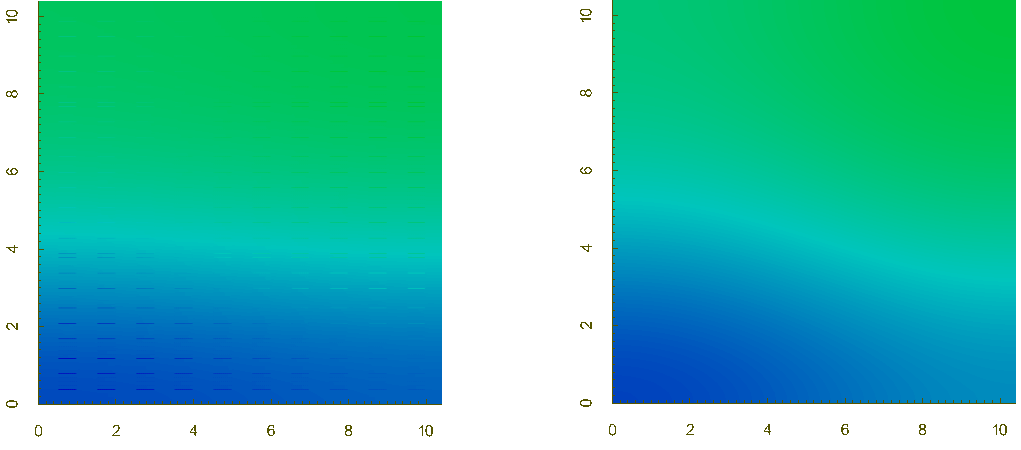
\includegraphics[height = 5.5 cm]{fig/numerical_example_MDE_exp1_400ms}} 
\subfigure[700 ms]{
    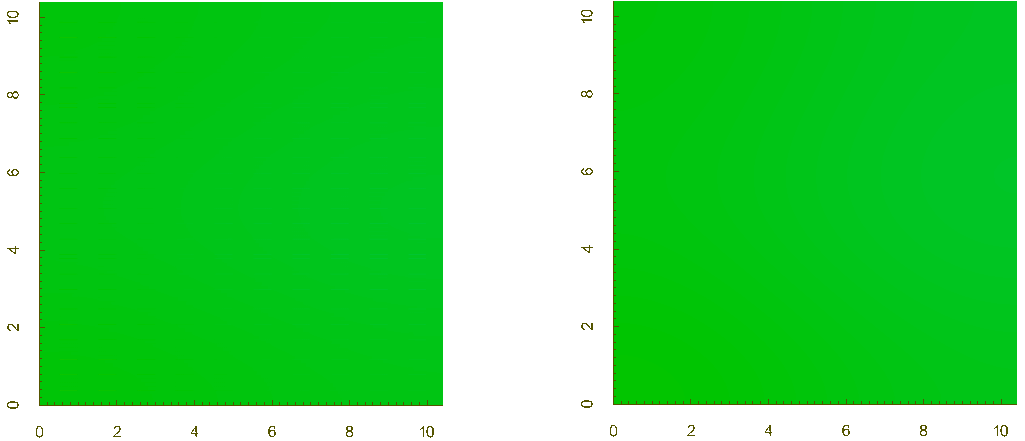
\includegraphics[height = 5.5 cm]{fig/numerical_example_MDE_exp1_700ms}}
\caption{temporal evolution of the solution for the exact problem (left) and homogenized problem (rigth)}\label{fig:mde_ex2}
\end{figure}


For the resolution of the linear exact problem was used the conjugate gradient method in addition with a pre-conditioner (AMG HYPRE: high performance pre-conditioner), while for the homogenized problem still was used the Gaussian elimination, due to the number of DOF's of it. Also, for both the exact and homogenized problem, the assemble of the matrix was done after the time loop, in order to increase performance.

\newpage
\subsubsection{Experiment \# 3: Very High Fibrosis on Small Domain}

\white{....} This second experiment is very similar to the first one, except that the amount of fibrotic tissue was increased to $\theta_c = 0.5$, and the domain was also increased to a $20 \times 20 [mm^2]$ square.

So, the results can be appreciated in the figure \ref{fig:mde_ex3}, and the asociated error in the figure \ref{fig:mde_ex3_error}. The computing time was as follow:

\begin{itemize}
\item Assemble of exact problem: 393.883 [seg]
\item Assemble of homogenized problem: 0.0595 [seg]
\item Total time for exact problem: 1338.2 seg
\item Total time for homogenized problem: 2,089 seg
\end{itemize}

\begin{figure}[H]
\centering
\subfigure{
    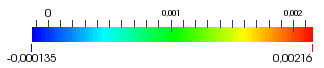
\includegraphics[height = 1.2 cm]{fig/numerical_example_MDE_exp3_colourbar}} \\
\subfigure[30 ms]{
    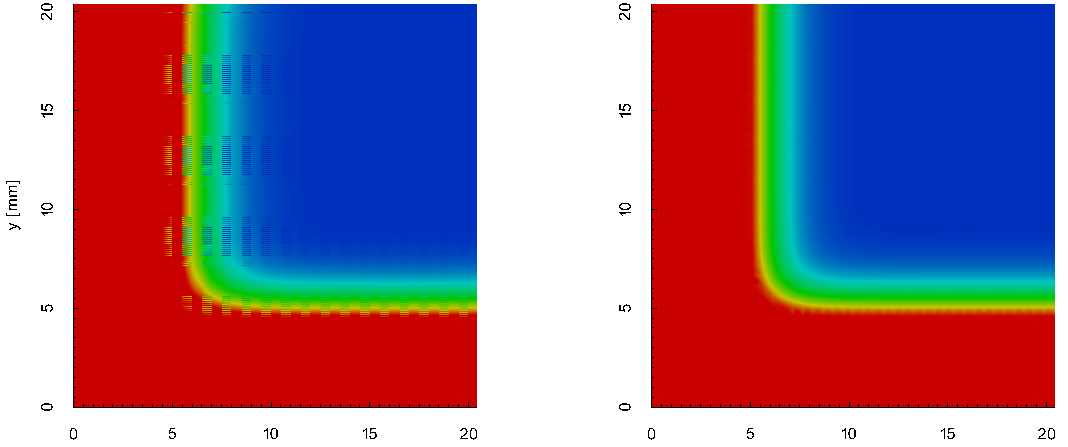
\includegraphics[height = 5.5 cm]{fig/numerical_example_MDE_exp3_20ms}} 
\subfigure[120 ms]{
    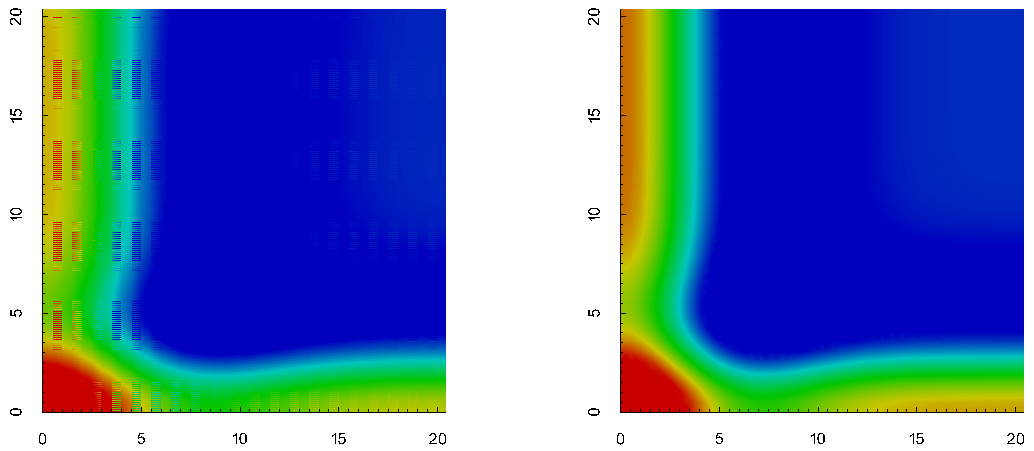
\includegraphics[height = 5.5 cm]{fig/numerical_example_MDE_exp3_200ms}}    
\end{figure}

\begin{figure}[H]
\centering
\subfigure[200 ms]{
    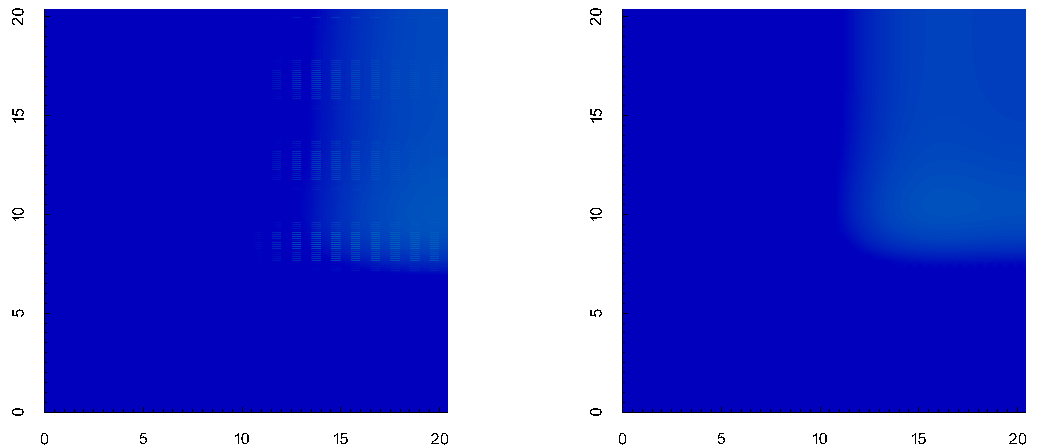
\includegraphics[height = 5.5 cm]{fig/numerical_example_MDE_exp3_600ms}}   
\subfigure[1000 ms]{
	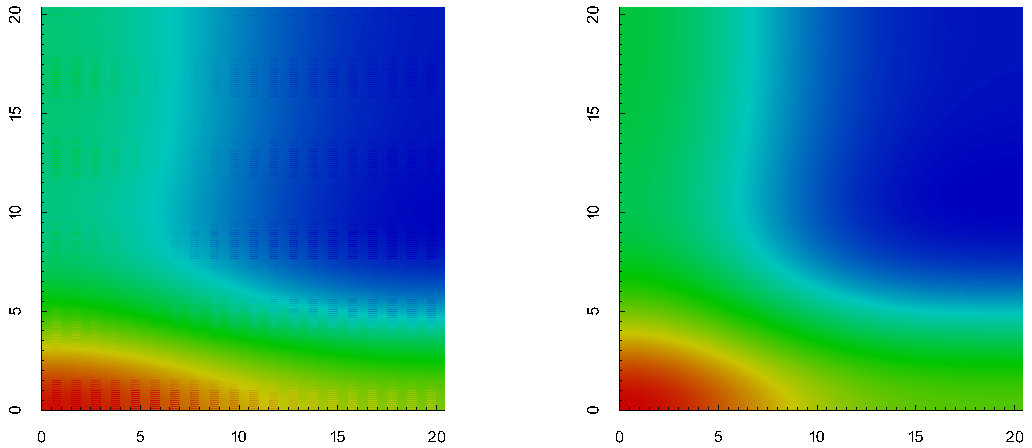
\includegraphics[height = 5.5 cm]{fig/numerical_example_MDE_exp3_1000ms}}
\caption{temporal evolution of the solution for the exact problem (left) and homogenized problem (rigth)}\label{fig:mde_ex3}
\end{figure}

\begin{figure}[H]
\centering
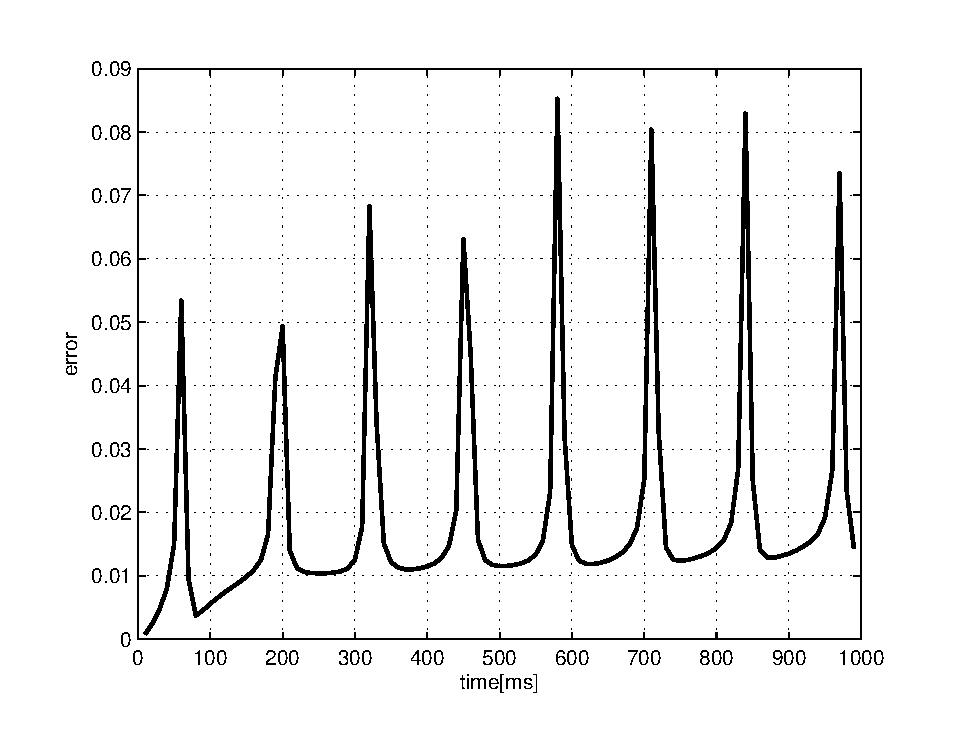
\includegraphics[height = 6.4 cm]{fig/numerical_example_MDE_exp3_error}
\caption{evolution of the error in time.}\label{fig:mde_ex3_error}
\end{figure}

The resolution of the linear systems was done in in the same way that the previous example, for both the exact and the homogenized problem.

\begin{figure}[H]
\centering
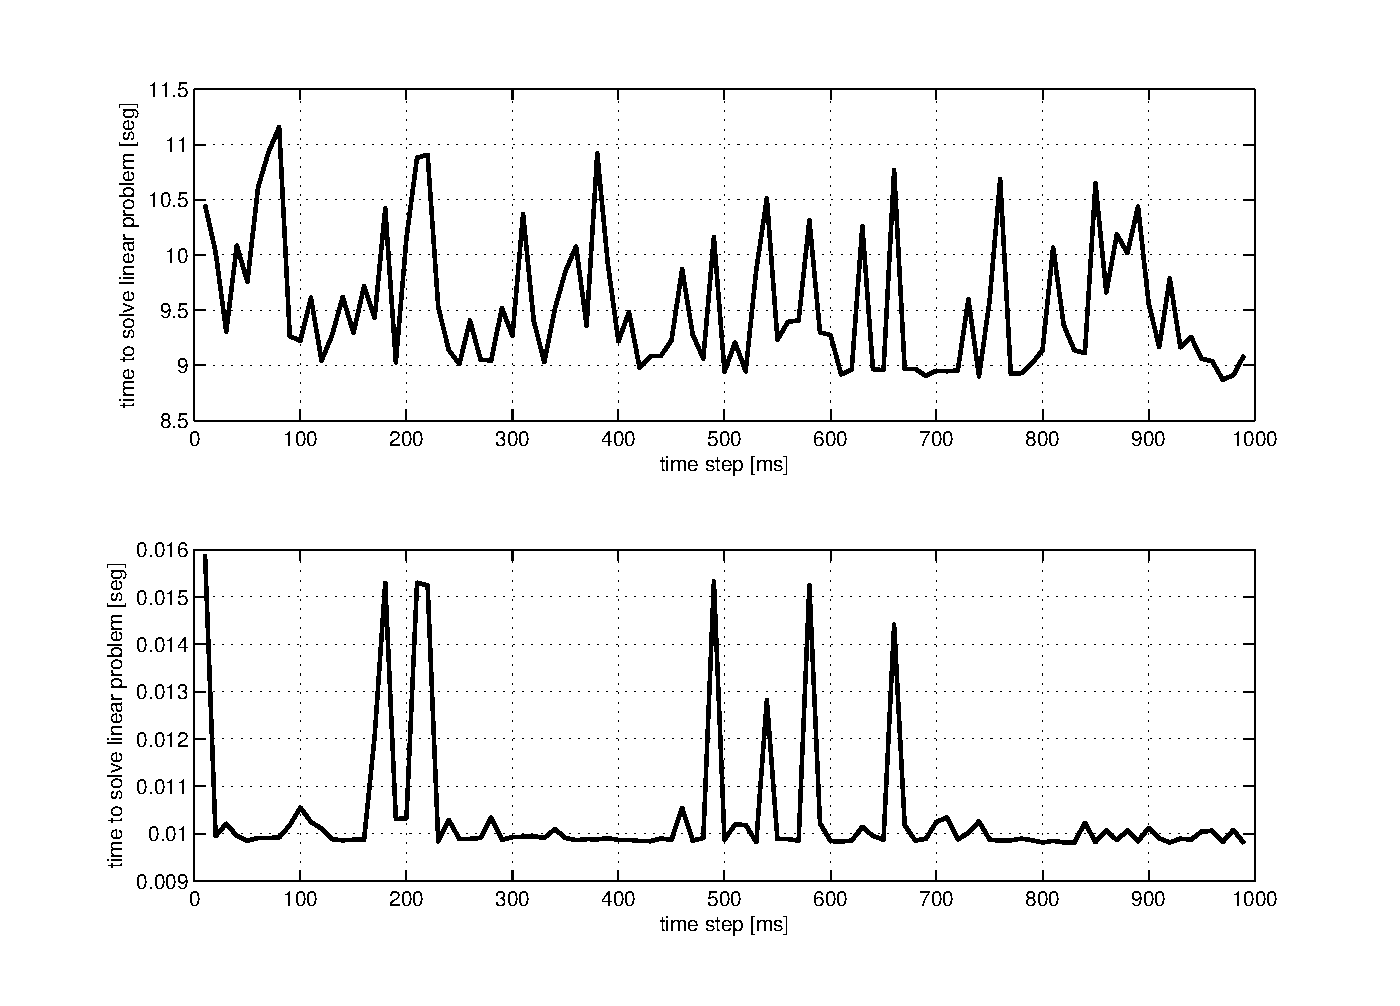
\includegraphics[height = 8 cm]{fig/numerical_example_MDE_exp3_benchmark}
\caption{evolution of the error in time.}
\end{figure}